% !TeX root = ../report.tex

In this study, there are two test cases. The first and the most simple one is that the media only consists of the markoil (start media in transducer). The second case is that the media consists of markoil and muscle. Solid media are not implement in this study yet. The resulted pressure only covers the area around actual focus of the transducer (Figure \ref{fig:sampling_box}). The initial intensity of every ray is the accurate value from far field approximation \ref{fig:ffa_profile}. However, error factor is introduced in the sampling process. Neither of the two methods to calculate contribution can produce genuine physics result. Hence, a scaling factor is required to scale the result back to the real world physics unit.

\begin{figure}[h]
    \centering
    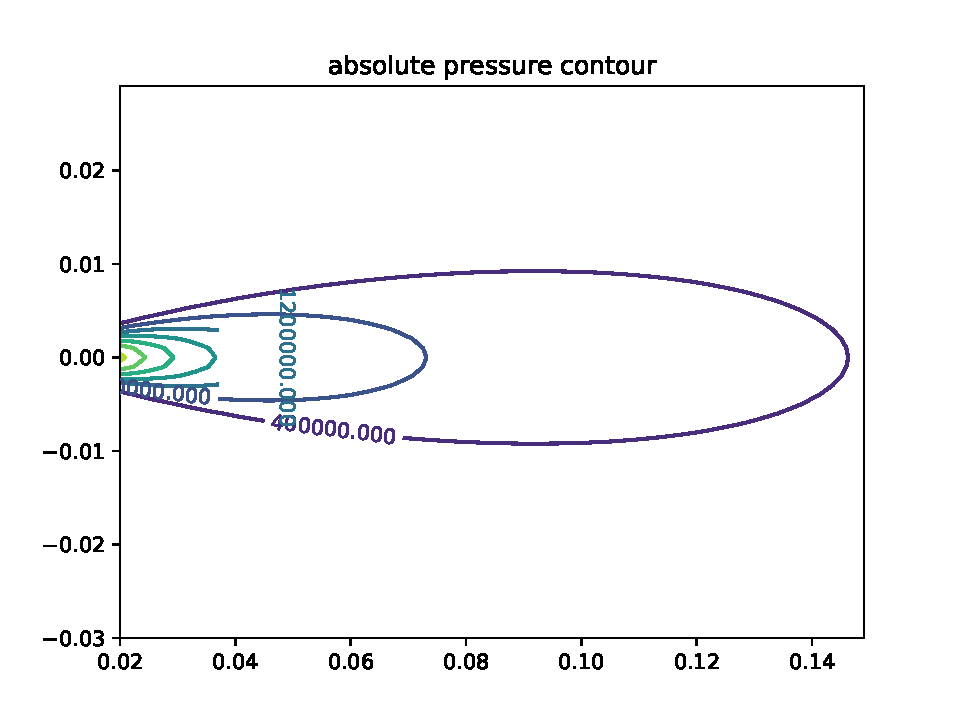
\includegraphics[width=0.4\textwidth]{ffa_profile}
    \caption{Far field approximation profile of one transducer element, start of $x$ axis is the minimal distance that far field holds. At the begining of every ray, the pressure is gained from the far field approxmiation.}
    \label{fig:ffa_profile}
\end{figure}

In this study, the result from Modena et al \cite{Modena_2018} is assumed as the ground truth. All the result from this study is compared against the ground truth. Despite the requirement of a scaling factor, however, the efforts in this study only try to prove that this method is possible for the first and the second test case. Hence, the comparison is based on similarity of the shape of the resulted pressure.

\begin{figure}[h]
    \centering
    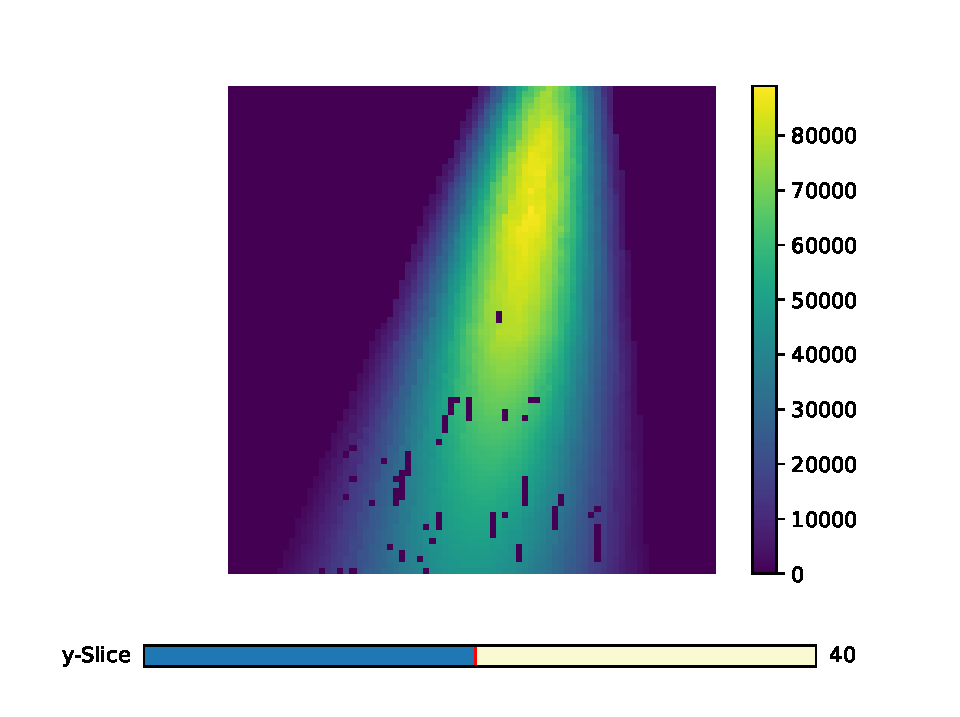
\includegraphics[width=0.55\textwidth]{one_transducer_highres}
    \caption{Pressure caused by one transducer. Blank point is due to that a small number of rays cannot cover all the area.}
    \label{fig:one_transducer_intensity}
\end{figure}

The ground truth is a matrix with the dimension of $75$ by $30$ by $30$. The result in this study is cropped to the same dimension to compare against ground truth. The similarity metric employed in the study is P-norm distance, in this case $p=3$.

\begin{equation} \label{eq:pnorm}
    D=\left(\sum_{i=0}^{n}|a_i - b_i|^p\right)^{1/p}
\end{equation}

In equation \ref{eq:pnorm}, $a_i$ stands for the result in this study and $b_i$ is the ground truth. An analysis of variance is performed on the three determining parameters of the result, number of rays, trident angle and theta (Section \ref{sec:components}).

The pressure is visualized as a heat map. First, we visualize the process of transmission and reflection of the ray origining from one transducer only (Figure \ref{fig:4reflection}). The color bar shows the pressure at the position. Figure \ref{fig:4reflection-a} show the state when the rays just emitted from the transducer element. It can be observed that the pressure suddenly decreases after passing through the interface. The rays reflected back into the markoils are discarded. Figure \ref{fig:4reflection-b} shows the state when the ray hits the second interface. It produces a nice illustration of reflection and refraction due to the large difference in speed of sound in the muscle and the bone. Figure \ref{fig:4reflection-c} and figure \ref{fig:4reflection-d} display the continued path of the reflected ray and refracted ray and their intersection with interfaces, respectively. When there's only one transducer element sending out rays, the pressure is always higher near the transducer. However, if all the transducer are activated, the superposition of all the transducer near the focus area will produce higher pressure.

\begin{figure}[h]
    \centering
    \begin{subfigure}[b]{0.45\textwidth}
        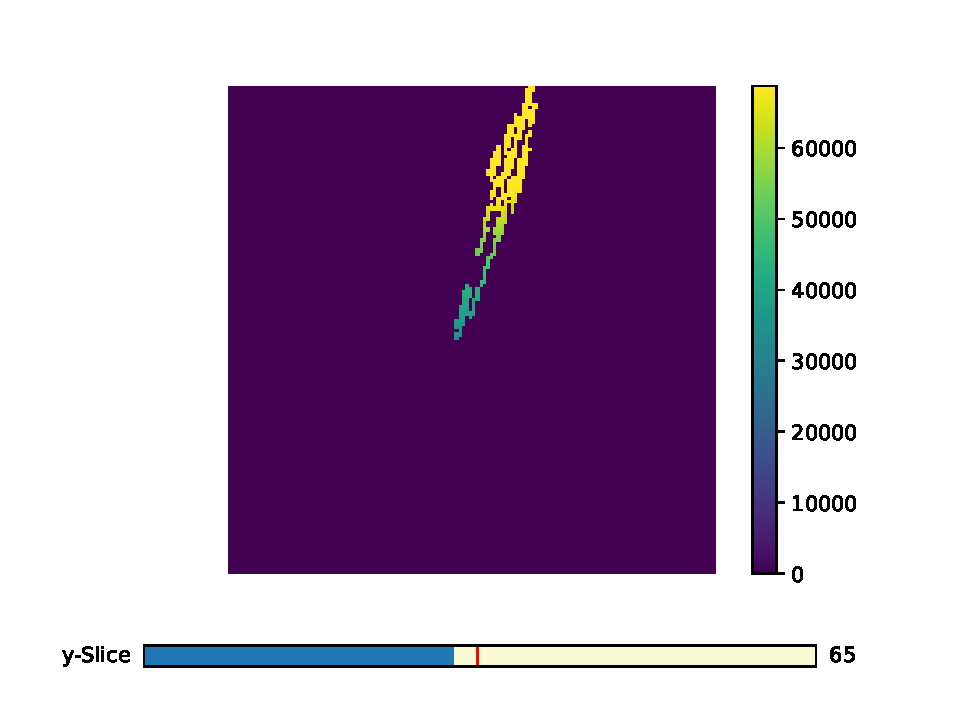
\includegraphics[width=\textwidth]{show_transmission1}
        \caption{no intersection}
        \label{fig:4reflection-a}
    \end{subfigure}
    ~ %add desired spacing between images, e. g. ~, \quad, \qquad, \hfill etc.
      %(or a blank line to force the subfigure onto a new line)
    \begin{subfigure}[b]{0.45\textwidth}
        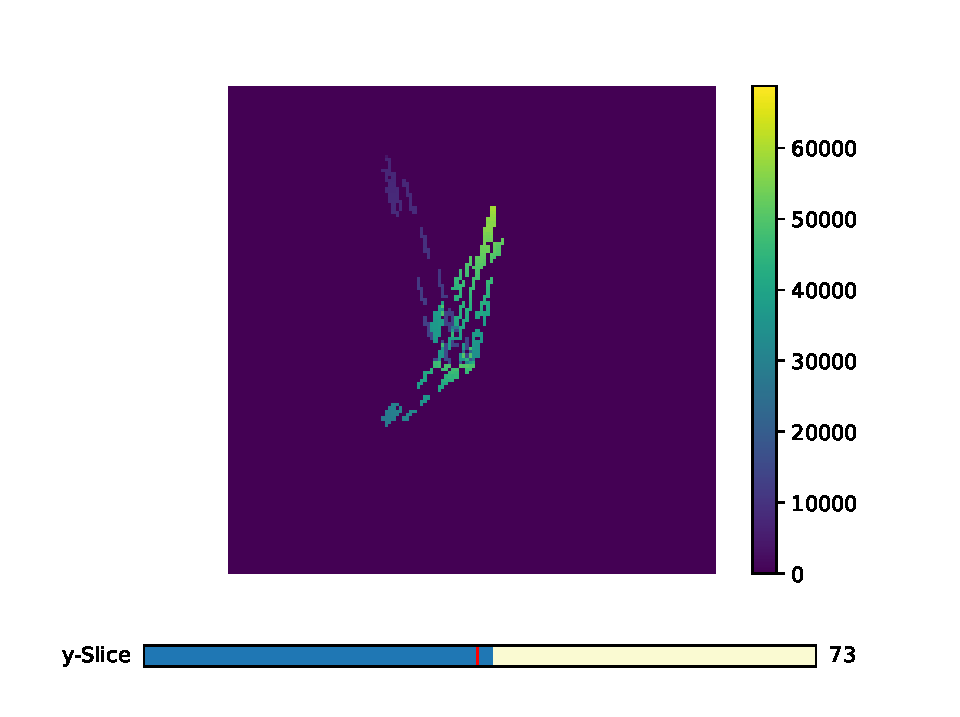
\includegraphics[width=\textwidth]{show_transmission2}
        \caption{one intersection with first interface}
        \label{fig:4reflection-b}
    \end{subfigure}
    ~ %add desired spacing between images, e. g. ~, \quad, \qquad, \hfill etc.
    %(or a blank line to force the subfigure onto a new line)
    \begin{subfigure}[b]{0.45\textwidth}
        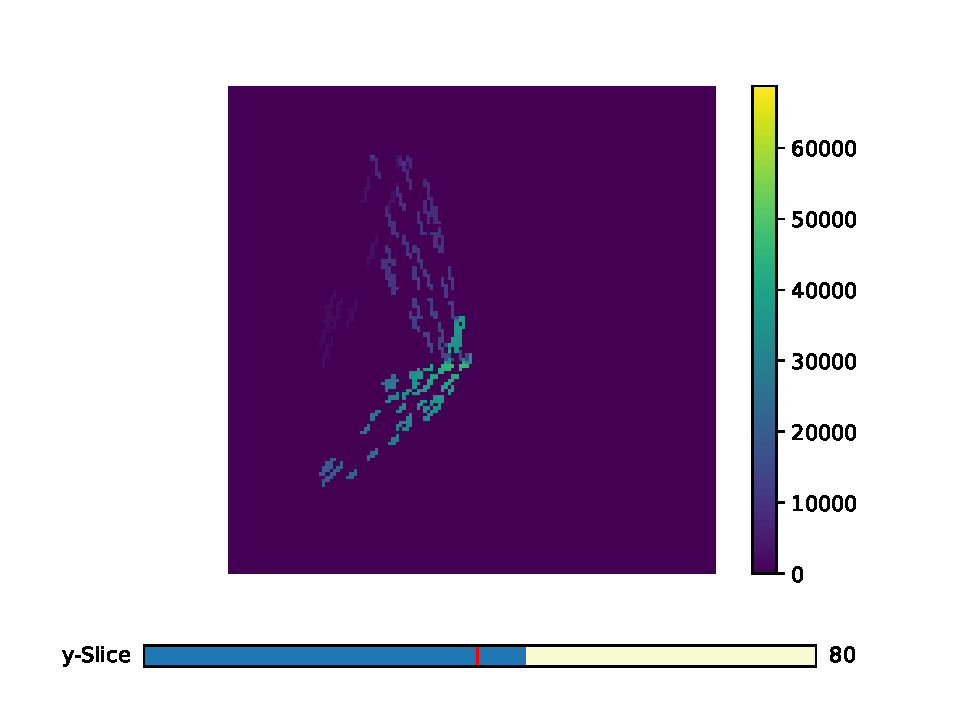
\includegraphics[width=\textwidth]{show_transmission3}
        \caption{continuation of new rays}
        \label{fig:4reflection-c}
    \end{subfigure}
    ~ %add desired spacing between images, e. g. ~, \quad, \qquad, \hfill etc.
    %(or a blank line to force the subfigure onto a new line)
    \begin{subfigure}[b]{0.45\textwidth}
        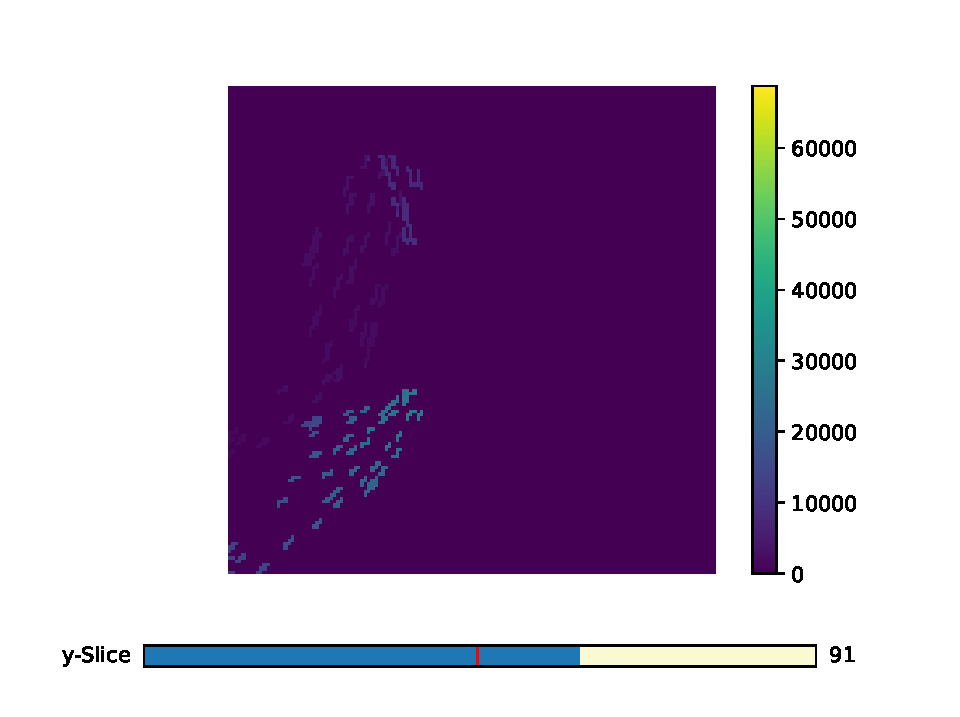
\includegraphics[width=\textwidth]{show_transmission4}
        \caption{second intersection}
        \label{fig:4reflection-d}
    \end{subfigure}
    \caption{Four moment during reflection and refraction. The slice number increases with the direction of the path of the trident.} \label{fig:4reflection}
\end{figure}

An advantage feature of ray tracing model is that it takes the interference of the wave into consideration. Wave interference is the superposition of two or more wave to form a wave of greater, lower or the same amplitude. In this study, the support of interference lies in the implementation of phase and pressure decay. The interference pattern proves the correctness of the model. As can be observed from Figure \ref{fig:interference-a}, the interference pattern is symmetric along the center axis. The interference pattern in Figure \ref{fig:interference-b} is centrosymmetric. Both of the two figures is consistent with the organization of the element on the transducer.

\begin{figure}[h]
    \centering
    \begin{subfigure}[b]{0.45\textwidth}
        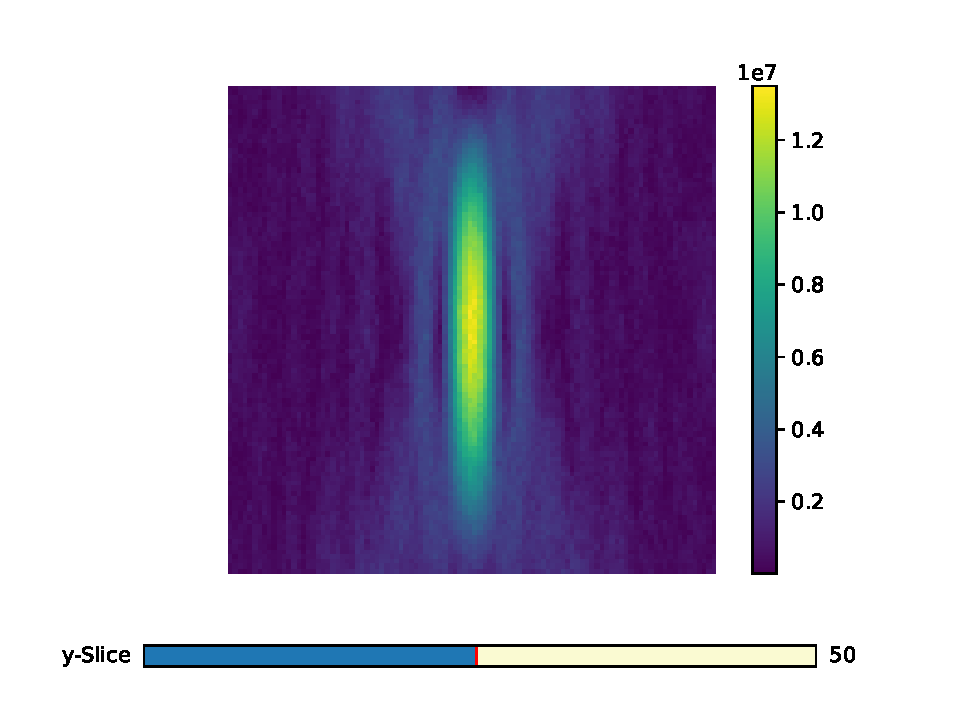
\includegraphics[width=\textwidth]{high_res}
        \caption{Slice along $y$ axis}
        \label{fig:interference-a}
    \end{subfigure}
    ~ %add desired spacing between images, e. g. ~, \quad, \qquad, \hfill etc.
      %(or a blank line to force the subfigure onto a new line)
    \begin{subfigure}[b]{0.45\textwidth}
        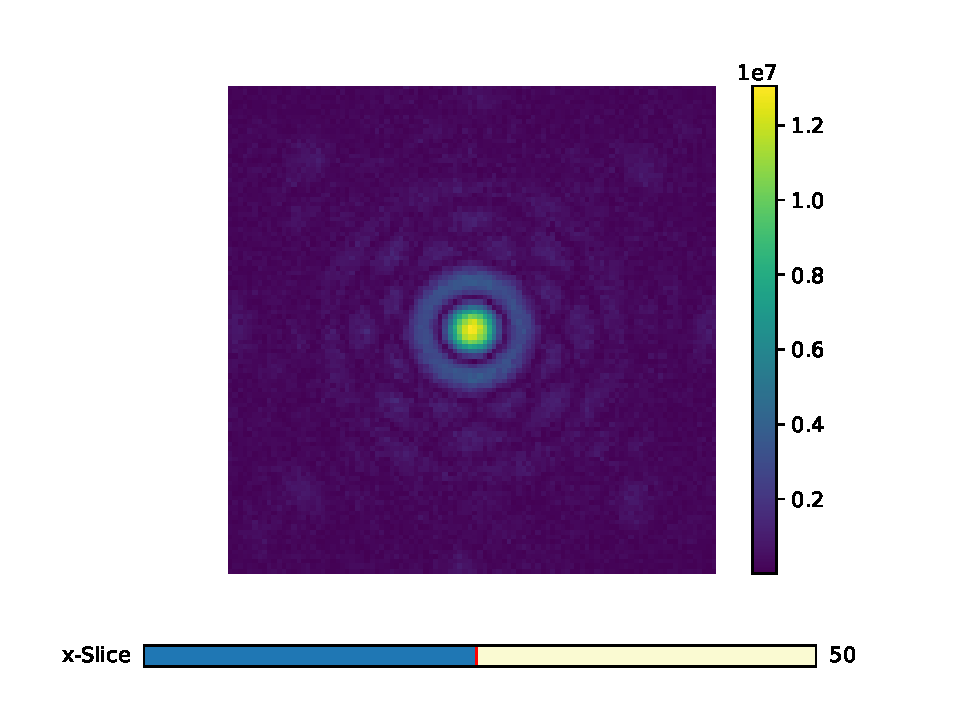
\includegraphics[width=\textwidth]{high_res_x}
        \caption{Slice along $x$ axis}
        \label{fig:interference-b}
    \end{subfigure}
    \caption{The focus area in case 1 (two media and one interface). The interference patterns can be observed.} \label{fig:interference}
\end{figure}

An experiment is set up to include three media in the geometry, markoil, muscle and bone. The actual focus area falls in the muscle, close to the muscle-bone interface. As a result, the pressure will include not only the interference between the rays casted from the transducer, but also the interference between incident rays and reflected rays at the focus areas. In Figure \ref{fig:3_med_interfered_focus}, the pressure at the focus area in this situation is displayed, in $-z$ direction in Figure \ref{fig:sampling_box}. Below the sampling window is the muscle-bone interface. Above the sampling window is the transducer. The interference between the incident rays and the reflected rays result in horizontal interference pattern, symmetric against a central plane. This can also prove the correctness of the ray casting model. 

\begin{figure}[h]
    \centering
    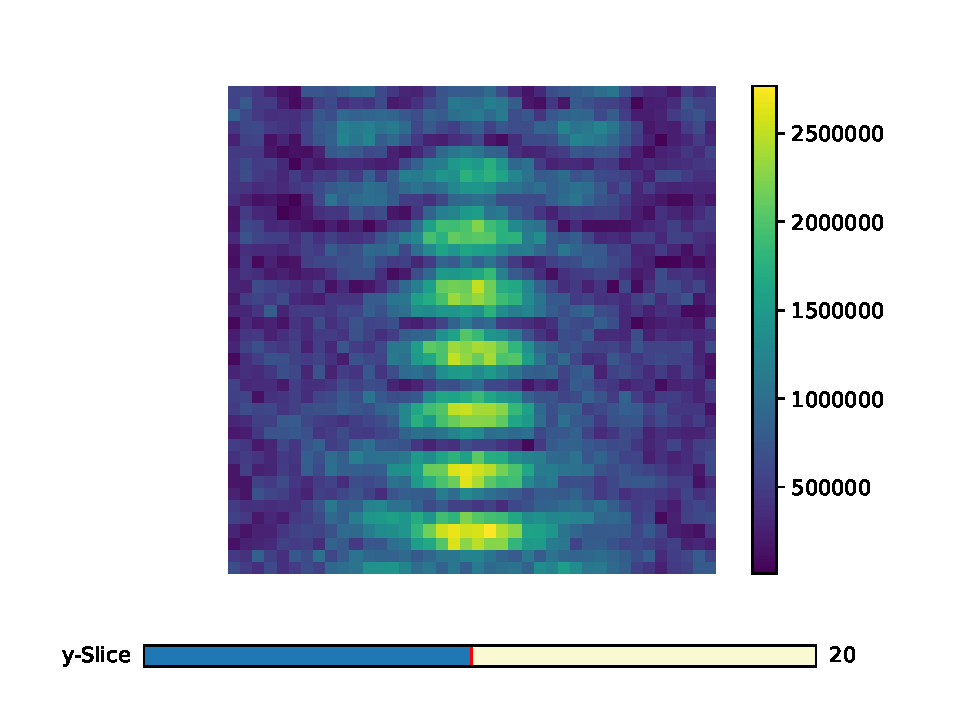
\includegraphics[width=0.55\textwidth]{3_med_interfered_focus}
    \caption{Pressure with more complex interference.}
    \label{fig:3_med_interfered_focus}
\end{figure}


The pressure can also be visualized as surface, which is also the method employed by Modena et al \cite{Modena_2018}. Figure \ref{fig:surface} show the surface plot of one slice of the pressure data sampled from the geometry (same data as Figure \ref{fig:interference-a}). Although the unit scale is different for the two surfaces, we can compare them based on how similar are these two surfaces. In Figure \ref{fig:surface}, the number of rays in both (a) and (b) are 20000. It can be observed that the method presented in this study produces a smoother result than the method by Modena et al \cite{Modena_2018}.

\begin{figure}[h]
    \centering
    \begin{subfigure}[b]{0.45\textwidth}
        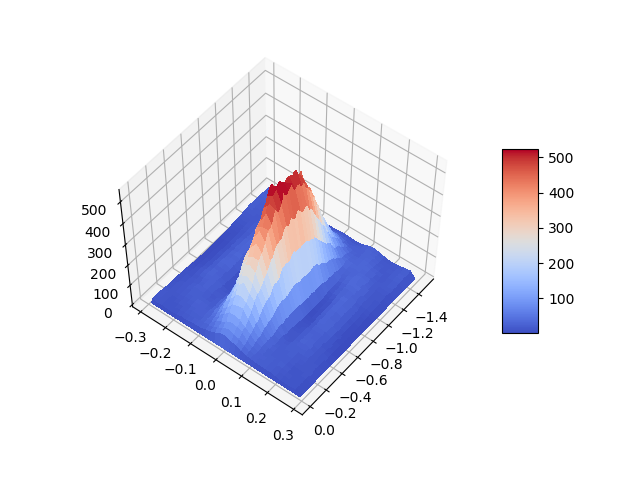
\includegraphics[width=\textwidth]{Daniela_et_al_surf}
        \caption{Result of Modena et al.}
        \label{fig:surface-a}
    \end{subfigure}
    ~ %add desired spacing between images, e. g. ~, \quad, \qquad, \hfill etc.
      %(or a blank line to force the subfigure onto a new line)
    \begin{subfigure}[b]{0.45\textwidth}
        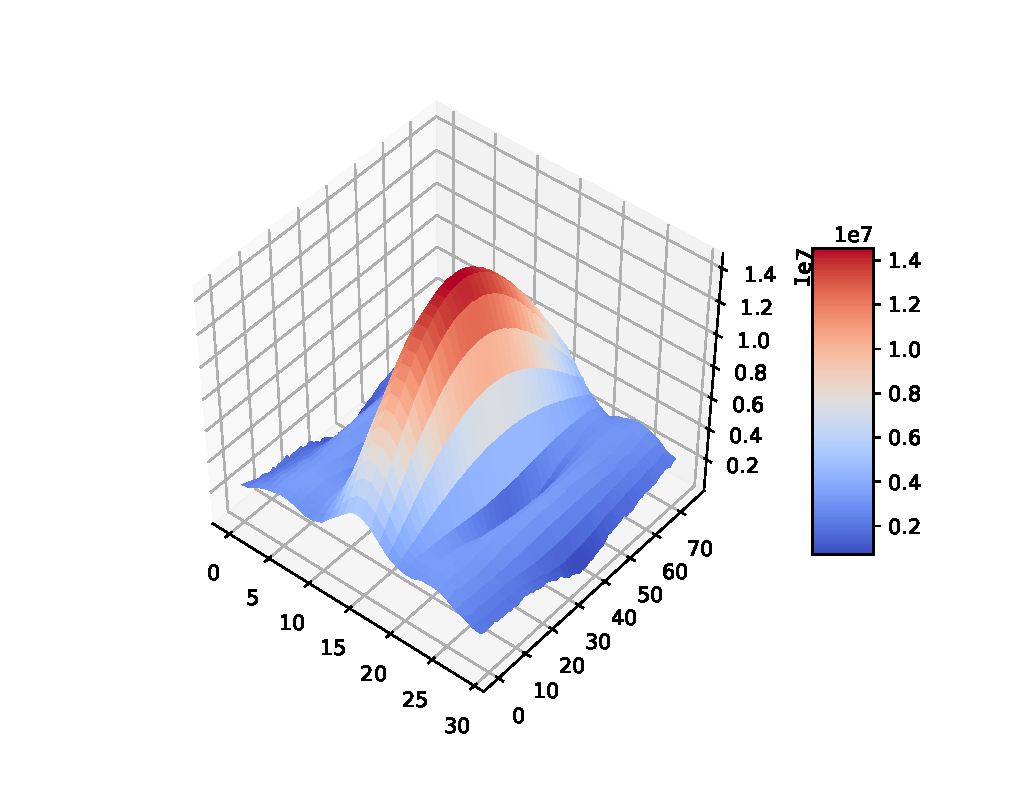
\includegraphics[width=\textwidth]{my_surf}
        \caption{Result in this study.}
        \label{fig:surface-b}
    \end{subfigure}
    \caption{The focus area in case 1 (two media and one interface). The interference patterns can be observed.} \label{fig:surface}
\end{figure}

To compare the similarity the result in this study with ground truth, three analysis of variance studies are conducted. There are many parameters which can affect the result. The most important three are number of rays $n\_rays$, theta max $\theta_{max}$ and trident angle. From previous study, it seems that more rays can yield better result. However, it also increases the computational time. To find an optimum number of rays which not only produces a result similar to the ground truth but also saves computational time, the number of rays is sampled in the range from 1000 to 20000 at the step of 500.

\begin{figure}[h]
    \centering
    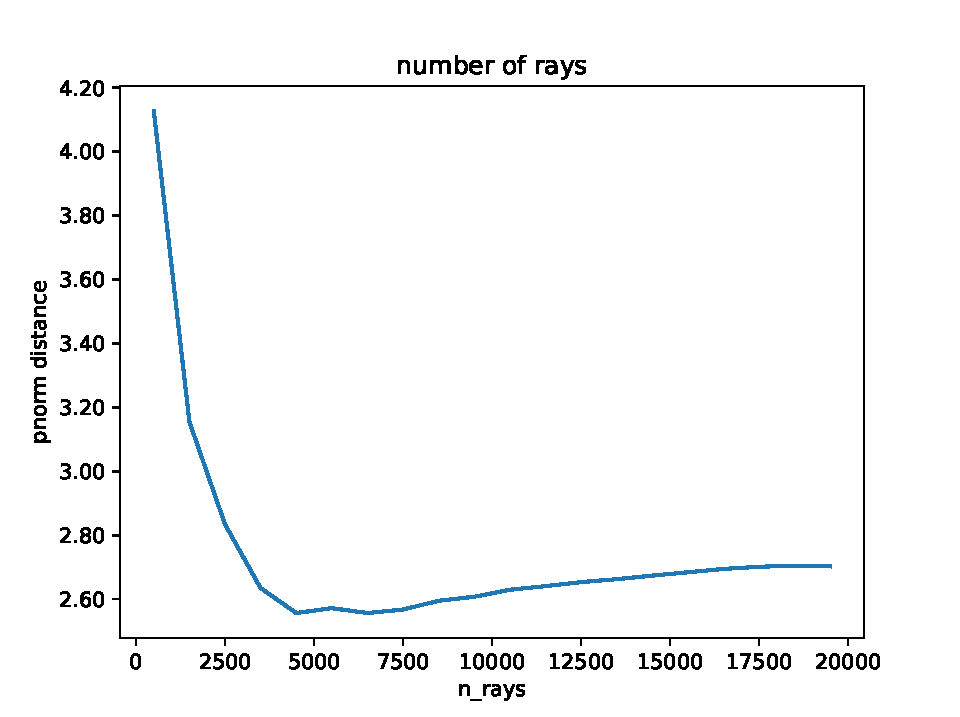
\includegraphics[width=0.6\textwidth]{anova_nrays}
    \caption{Analysis of parameter $n\_rays$.}
    \label{fig:anova_nrays}
\end{figure}

The similarity metric is calculated for each number of rays (Figure \ref{fig:anova_nrays}). The 3-norm distance is minimal at around $n\_rays=4500$. The less the distance is, the more similar the result in this study is to the ground truth. Before $n\_rays=4500$, the distance drastically decreases. After $n\_rays=4500$, the distance increases at a slower pace. This phenomenon can be interpreted as that the trident ray method produces the result most similar to the ground truth at $n\_rays=4500$. When $n\_rays$ is more than $4500$, the trident ray method can producer even smoother result than the ground truth (Figure \ref{fig:surface}). In the following experiments, the number of rays is 4500. 

Theta max $\theta_{max}$ determines the spreading angle of the rays from one transducer element. When the number of rays is determined, smaller spreading angle can cast more rays to the focus area. However, $\theta_{max}$ is also required to be large enough to make sure that every cube in the sampling box is covered. A similar study is conducted for parameter $\theta_{max}$. $\theta_{max}$ is incremented from $0.01$ to $0.1$, $0.01$ at each step (Figure \ref{fig:anova_theta_max}). Similarly, the distance plot is very similar to that of $n\_rays$. The minimal distance is achieve at $\theta_{max}=0.05$. From $\theta_{max}=0.01$ till $\theta_{max}=0.03$, the distance decreases faster. This is due to that the $\theta_{max}$ is too small to cover the entire sampling space. In the next study, $\theta_{max}=0.05$ is used as the optimal value.

\begin{figure}[h]
    \centering
    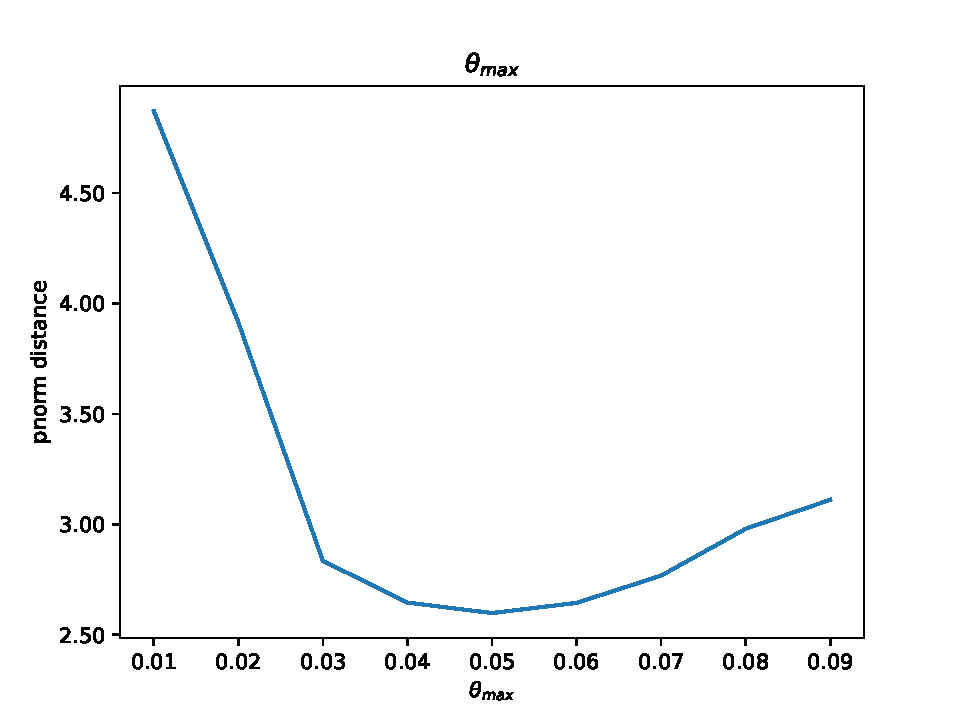
\includegraphics[width=0.6\textwidth]{anova_theta_max}
    \caption{Analysis of parameter $\theta_{max}$.}
    \label{fig:anova_theta_max}
\end{figure}

\begin{figure}[h]
    \centering
    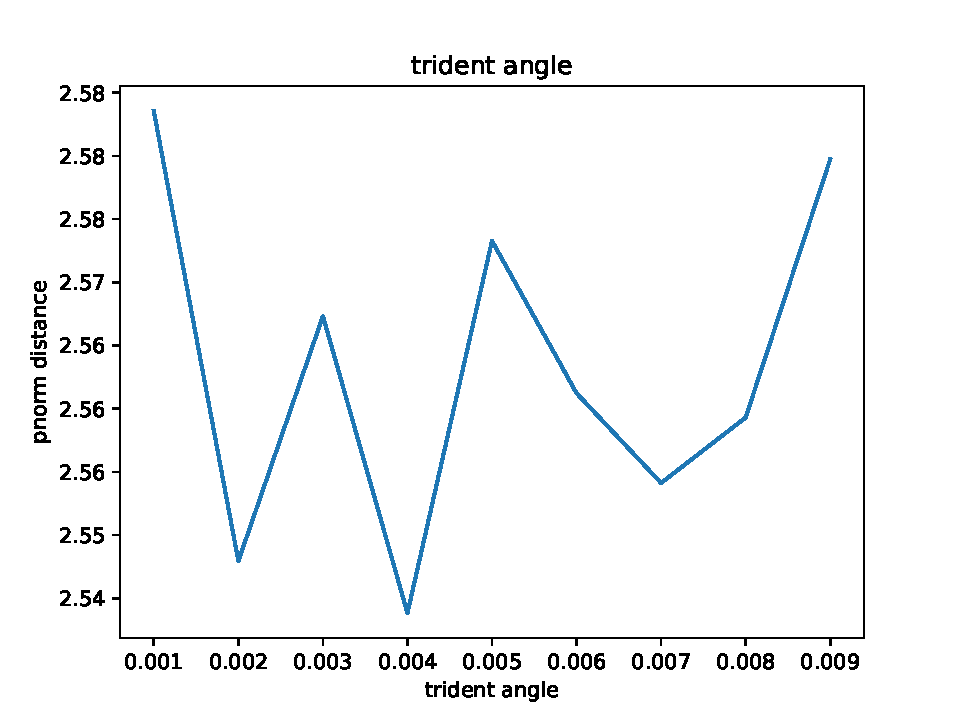
\includegraphics[width=0.6\textwidth]{anova_trident_angle}
    \caption{Analysis of parameter trident angle.}
    \label{fig:anova_trident_angle}
\end{figure}

Theta max $\theta_{max}$ determines the spreading angle of the rays from one transducer element. When the number of rays is determined, smaller spreading angle can cast more rays to the focus area. However, $\theta_{max}$ is also required to be large enough to make sure that every cube in the sampling box is covered. A similar study is conducted for parameter $\theta_{max}$. $\theta_{max}$ is incremented from $0.01$ to $0.1$, $0.01$ at each step (Figure \ref{fig:anova_theta_max}). Similarly, the distance plot is very similar to that of $n\_rays$. The minimal distance is achieve at $\theta_{max}=0.05$. From $\theta_{max}=0.01$ till $\theta_{max}=0.03$, the distance decreases faster. This is due to that the $\theta_{max}$ is too small to cover the entire sampling space. In the next study, $\theta_{max}=0.05$ is used as the optimal value.

The third parameter to be analysed is the angle between the power ray and the auxiliary ray within a trident. Figure \ref{fig:anova_trident_angle} shows the result of analysis of trident angle. However, it doesn't show any evidence of an optimal value. The experiment in this study uses 0.005 as the optimal trident angle.
